\section{关键组件的可及性与首次见齐时间}\label{sec:access}
\subsection{联合抽取概率与关键牌复制}
令三个互不重叠的必需类别数量为$m_1=a,m_2=b,m_3=k$，
其中C类问题取$k=c$，E类问题取$k=c+d$。
记$F_n$为三类各至少出现一张的事件。
对“遗漏某一类”的事件应用容斥，得到
\begin{equation}\label{eq:inclusion}
\Prob(F_n)=\sum_{J\subseteq\{1,2,3\}}(-1)^{|J|}
\frac{\binom{N-\sum_{j\in J}m_j}{n}}{\binom Nn}.
\end{equation}
约定上参数为负或下参数越界的组合数为0。
该式统一覆盖不同副本数量；也可通过枚举三类在前缀中的正计数得到相同的组合概率。

当$a=b=1$时，可先强制A、B进入前缀，再从其余$N-2$张中排除不含触发牌的子集：
\begin{equation}\label{eq:singleton}
\Prob(F_n)=
\frac{\binom{N-2}{n-2}-\binom{N-2-k}{n-2}}{\binom Nn}.
\end{equation}
由此，基准前10张的两种可及性分别为
\begin{equation}\label{eq:baseline-access}
\Prob(F_{10}^C)=\frac{25}{253}\approx0.098814,\qquad
\Prob(F_{10}^E)=\frac{63}{506}\approx0.124506.
\end{equation}
E类还允许D充当消耗组件，因此$F_n^C\subseteq F_n^E$，对应的可及性更高。

\begin{figure}[htbp]
\centering
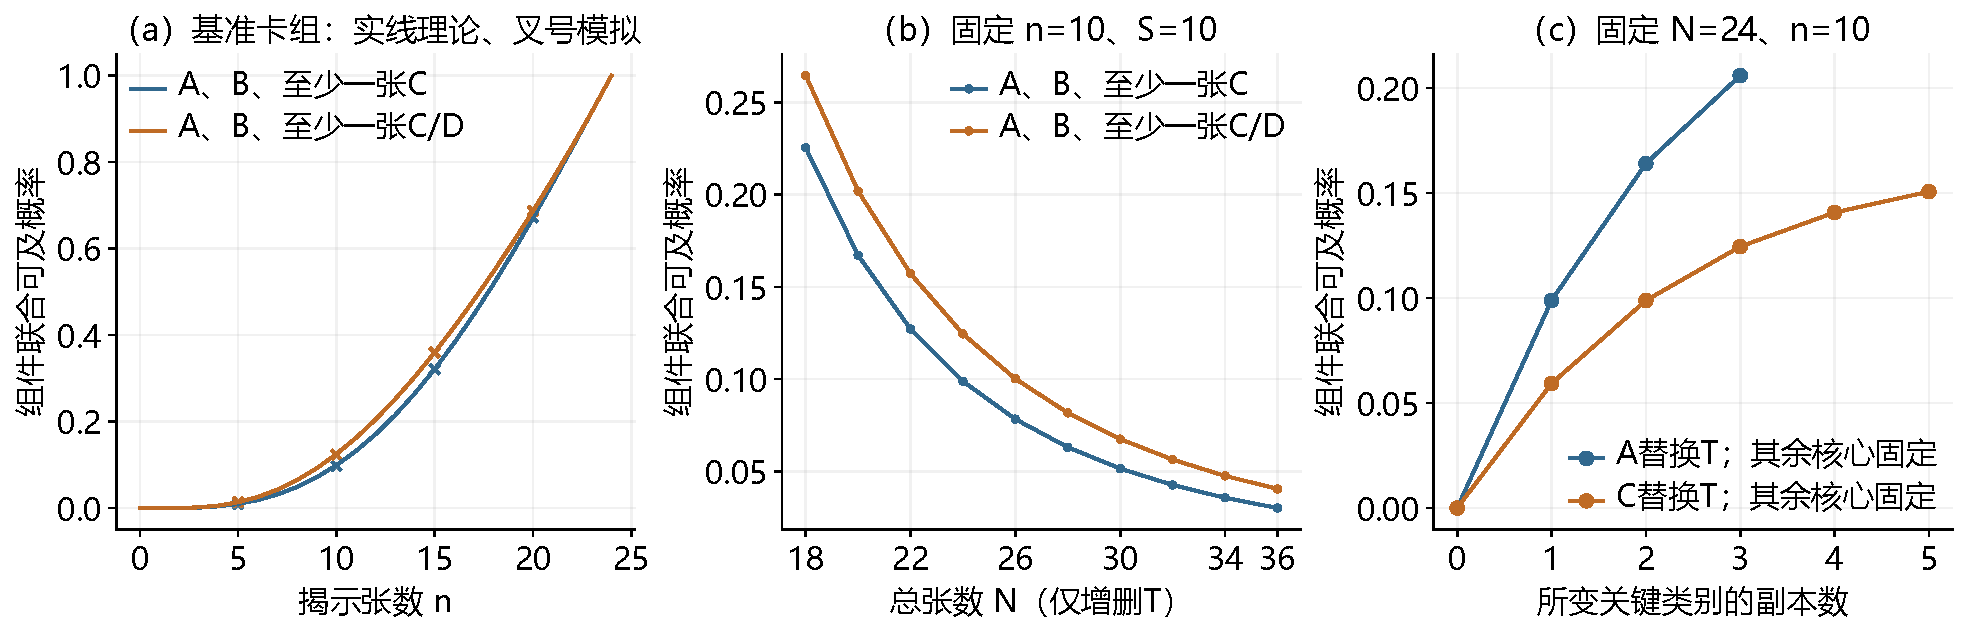
\includegraphics[width=\linewidth]{01_accessibility.pdf}
\caption{联合组件可及性。实线为精确理论值，左图叉号为每配置20万次排列模拟；
改变$N$通过增删T实现，复制关键牌通过固定$N$替换T实现。}\label{fig:access}
\end{figure}

图\ref{fig:access}中，可及性随观察预算$n$增加而上升；
固定核心数量而增加普通牌，会稀释固定前缀中的组件机会。
这两点也可通过同一随机排列中的插入或前缀延伸耦合证明。
对于$F_n^C$，固定$N,n,a=b=1$，并将一张非必需类别牌替换为C，
使C的数量由$c$增至$c+1$。由式\eqref{eq:singleton}与帕斯卡恒等式可得：
\begin{equation}\label{eq:marginal}
\Prob(F_n^C;c+1)-\Prob(F_n^C;c)
=\frac{\binom{N-3-c}{n-3}}{\binom Nn}.
\end{equation}
该增量随$c$非增，表明固定规模下复制C的边际收益递减。
若直接增加卡牌，总数$N$也随之变化；对$F_n^E$则以$c+d$为有效触发数，
例如把D替换为C时，$c+d$保持不变。

\subsection{首次见齐时间的分布与矩}
用$\tau_C,\tau_E$表示两类事件的首次见齐位置。
对任一类事件，令$\tau=\min\{n:F_n\text{成立}\}$。
当必需类别均存在时，$F_n$随$n$单调，因而
\begin{equation}\label{eq:time-pmf}
\Prob(\tau\le n)=\Prob(F_n),\qquad
\Prob(\tau=n)=\Prob(F_n)-\Prob(F_{n-1}).
\end{equation}
由逐样本恒等式$\tau=\sum_{n=0}^{N-1}\ind_{\{\tau>n\}}$及
$\tau^2=\sum_{n=0}^{N-1}(2n+1)\ind_{\{\tau>n\}}$，有
\begin{equation}\label{eq:tail-moments}
\E(\tau)=\sum_{n=0}^{N-1}\Prob(\tau>n),\qquad
\E(\tau^2)=\sum_{n=0}^{N-1}(2n+1)\Prob(\tau>n).
\end{equation}
再减去$\E(\tau)^2$即得方差。分位数统一取
$q_\alpha=\min\{n:\Prob(\tau\le n)\ge\alpha\}$。
基准精确结果见表\ref{tab:time}，其中
$\E(\tau_E)=205/12$、$\V(\tau_E)=25565/1008$，
$\E(\tau_C)=35/2$、$\V(\tau_C)=275/12$。

\begin{table}[htbp]
\centering\small
\caption{基准首次见齐时间的精确理论指标}\label{tab:time}
\begin{tabular}{lrrrrr}
\toprule
时间 & $\mathbb E(\tau)$ & $\operatorname{Var}(\tau)$ & $q_{0.5}$ & $q_{0.9}$ & $q_{0.95}$ \\
\midrule
$\tau_C$ & 17.500000 & 22.916667 & 18 & 23 & 24 \\
$\tau_E$ & 17.083333 & 25.362103 & 18 & 23 & 24 \\
\bottomrule
\end{tabular}

\end{table}

E类的均值较小，方差却较大，两类90\%分位数均为23张。
由于逐样本有$\tau_E\le\tau_C$，增加备选消耗组件缩短了平均见齐时间，
却使方差增大，体现出均值与离散程度的不同变化。
将容斥代入尾和，还可得到
\begin{equation}\label{eq:time-general-mean}
\E(\tau)=(N+1)
\sum_{\varnothing\ne J\subseteq\{1,2,3\}}
\frac{(-1)^{|J|+1}}{1+\sum_{j\in J}m_j}.
\end{equation}
这里使用恒等式
$\sum_{n=0}^{N-1}\binom{N-m}{n}/\binom Nn=(N+1)/(m+1)$；
右侧也等于$m$个指定位置的最小次序统计量期望。
固定关键类别数量时，首次见齐时间的期望与$N+1$成正比。

\subsection{有限前缀中的顺序约束}
仍取$a=b=1$。令$j$为A、B位置中较后者，则
$\Prob(\max(\operatorname{pos}A,\operatorname{pos}B)=j)
={2(j-1)}/{[N(N-1)]}$。
给定这两位置，$k$张触发牌均匀占据其余$N-2$个位置。
前缀中可满足顺序的位置为$j+1,\ldots,n$，共有$n-j$个。
用补集排除这些位置没有触发牌的情况，得
\begin{equation}\label{eq:order}
\Prob(O_n)=\sum_{j=2}^{n-1}\frac{2(j-1)}{N(N-1)}
\left[1-\frac{\binom{N-2-(n-j)}{k}}{\binom{N-2}{k}}\right].
\end{equation}
抽完整副牌时，$k+2$张关键牌的最后一张属于触发类的概率为
$\Prob(O_N)=k/(k+2)$。对有限前缀则用式\eqref{eq:order}计入触发牌实际出现数量。

\begin{figure}[htbp]
\centering
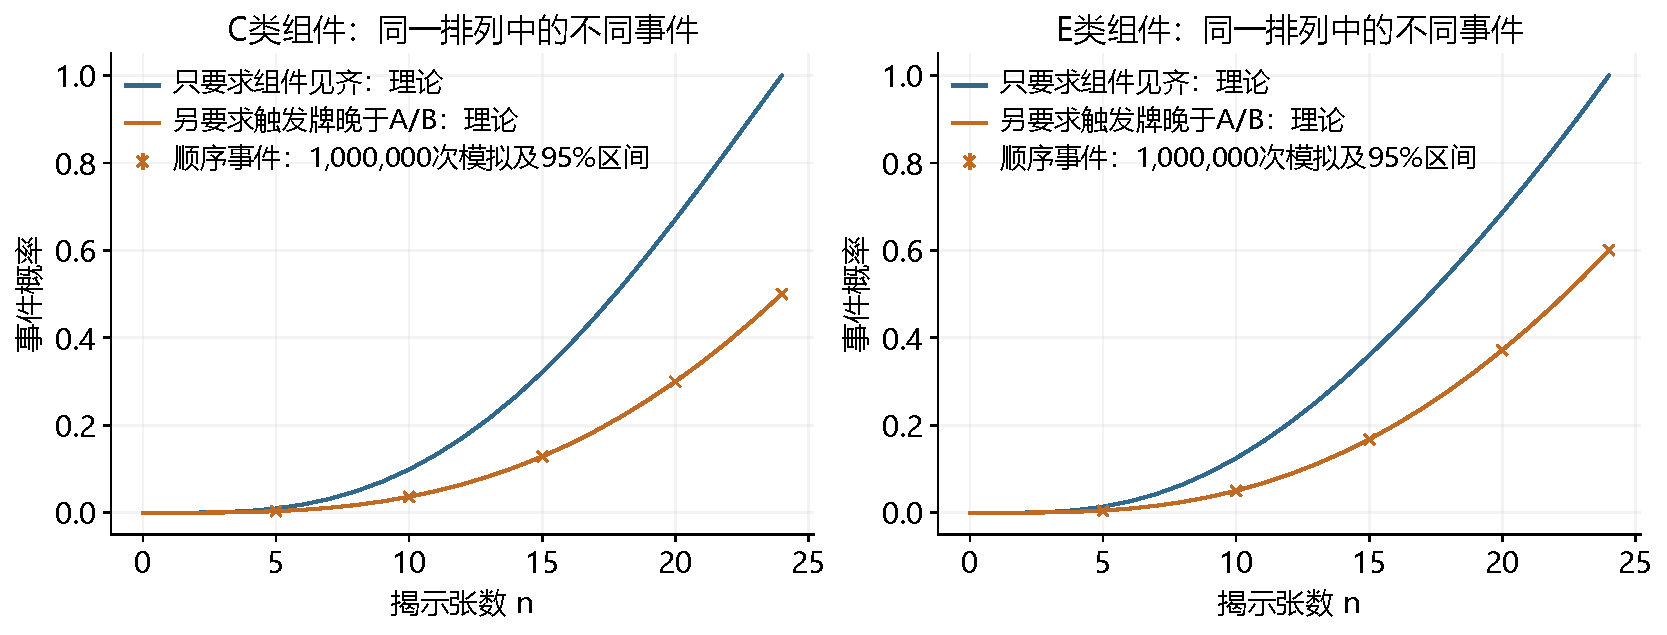
\includegraphics[width=\linewidth]{03_order_constraint.pdf}
\caption{组件见齐与顺序事件的精确概率；叉号及95\% Wilson区间来自独立100万次排列模拟。}\label{fig:order}
\end{figure}

基准$n=10$时，$\Prob(O_{10}^C)=5/138\approx0.036232$，
$\Prob(O_{10}^E)=1/20=0.05$，分别为相应无序概率的36.67\%和40.16\%。
图\ref{fig:order}显示：即使抽完整副牌，无序事件概率达到1，
特定顺序事件的概率仍为$1/2$或$3/5$。
两种曲线的差距直观体现了抽牌次序对组件协同的影响。
